
\documentclass[a4paper,UKenglish,cleveref, autoref]{oasics-v2019}

\bibliographystyle{plainurl}
\usepackage{booktabs}
\usepackage{fancyvrb}
\fvset{fontsize=\small,commandchars=\\\{\}}


\def\ourtitle{Musikla: Language for Generating Musical Events}
\title{\ourtitle}
\titlerunning{\ourtitle}

\author{Pedro M. Silva}{Departamento de Informática, Universidade do Minho, Braga, Portugal}{pg38423@alunos.uminho.pt}{}{}

\author{José João Almeida}%
       {Algoritmi, Departamento de Informática, Universidade do Minho, Braga, Portugal}%
       {jj@di.uminho.pt}%
       {https://orcid.org/0000-0002-0722-2031}
       {}

\authorrunning{Pedro M. Silva and J.\,J. Almeida}
\Copyright{Pedro Miguel Silva, José João Almeida}

\begin{CCSXML}
<ccs2012>
<concept>
<concept_id>10010147.10010178.10010179.10010186</concept_id>
<concept_desc>Computing methodologies~Language resources</concept_desc>
<concept_significance>500</concept_significance>
</concept>
</ccs2012>
\end{CCSXML}

\ccsdesc[500]{Computing methodologies~Language resources}

\keywords{Domain Specific Language, Music Notation, Interpreter, Programming Language}

%\nolinenumbers %uncomment to disable line numbering

%Editor-only macros:: begin (do not touch as author)%%%%%%%%%%%%%%%%%%%%%%%%%%%%%%%%%%
\EventEditors{John Q. Open and Joan R. Access}
\EventNoEds{2}
\EventLongTitle{42nd Conference on Very Important Topics (SLATE 2020)}
\EventShortTitle{SLATE 2020}
\EventAcronym{SLATE}
\EventYear{2020}
\EventDate{December 24--27, 2020}
\EventLocation{Little Whinging, United Kingdom}
\EventLogo{}
\SeriesVolume{42}
\ArticleNo{23}
%%%%%%%%%%%%%%%%%%%%%%%%%%%%%%%%%%%%%%%%%%%%%%%%%%%%%%

\begin{document}

\maketitle

\begin{abstract}
  In this paper, we'll discuss a simple approach to integrating musical events, such as notes or chords, into a programming language. This means treating music sequences as a first class citizen. It will be possible to save those sequences into variables or play them right away, pass them into functions or apply operators on them (like transposing or repeating the sequence). Furthermore, instead of just allowing static sequences to be generated, we'll integrate a music keyboard system that easily allows the user to bind keys (or other kinds of events) to expressions. Finally, it is important to provide the user with multiple and extensible ways of outputing their music, such as synthesizing it into a file or directly into the speakers, or writing a MIDI or music sheet file. We'll structure this paper first with an analysis of the problem and its particular requirements. Then we will discuss the solution we developed to meet those requirements. Finally we'll analyze the result and discuss possible alternative routes we could've taken.
\end{abstract}

\section{Introduction}
Musikla stands for Music and Keyboard Language. Our goal is to develop a DSL (\textit{Domain Specific Language}) that allows treating musical events with the same importance as other basic types, like integers and booleans, are treated in most programming languages. More than generating these musical events offline, we want to be able to easily declare keyboards that map keys to expressions that either mutate the state or play musical events (or even both).

The project can be partitioned in three different, modular layers: inputs, the language, and outputs. While music events can be described as code literals inside our language, they can also originate from many other sources (such as files or physical devices such as pianos). After being processed by our language, they are then emitted as a stream of musical events to the \textbf{Player} component, which then multiplexes those events into however many outputs the user defined.

\begin{figure}[ht]
  \centering
  {%
  \setlength{\fboxsep}{0pt}%
  \setlength{\fboxrule}{0pt}%
  \fbox{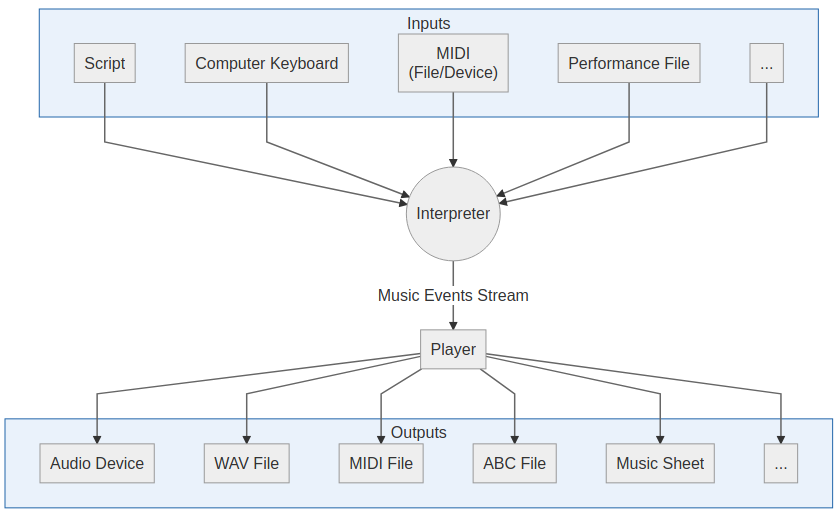
\includegraphics[width=.65\linewidth]{../dissertation/rpd/img/diagram_architecture_en_vertical.png}}%
  }%
  \caption{The three main layers of the project.}
  \label{fig:architecture}
\end{figure}

While the development of both the input and output layers, as well as their many respective components, presents by itself many interesting challenges that could be discussed, we will instead focus this paper on the aspects of the middle layer: the \textit{interpreter}, while ackowledging the existence (and their effects) of the layers that wrap around it.

As such, the problem of developing the interpreter can be divided into two parts: the syntax used for describing the notes and the operators that compose them inside the language; and the semantics of the generated events, how they are stored in memory, and how their temporal properties (start time and duration) are handled without forcing the programmer/user to always manually type them. 

Designing the syntax for describing those musical expressions, especially given our strong desire to make those musical expressions first class citizens like other primitive data types in most programming languages (such as numbers, strings or arrays are), did unearth some challenges. To minimize the learning curve for new users, and avoid reinventing the wheel, we decided to adopt a subset of the very popular note declaration syntax from the ABC Notation project\cite{AbcNotation, AbcPlus} and integrate it with our language.

As for the execution model, we decided to go with a tree-walker interpreter\cite{CraftingInterpreters}. Altough computationally slower than other alternatives (such as a bytecode virtual machine), the ease of implementation allowed us to prototype and develop features extremely fast. And with a more mature and stable language in the future, there is always the potential to rewrite the interpreter if performance or latency ever reveal themselves as potential problems.


The simplest way of generating such musical events in a programming language is to use already common, \textit{low-level}, programming mechanisms, such as using a procedural approach where the user creates each event manually by calling a function and providing as parameters all the events' information, such as it's timestamp and duration. This is the approach used by some of the existing languages in this space, such as \textit{SonicPi}\cite{Aaron2014TemporalSF}, and it's usage can somewhat resemble the code in listing~\ref{lst:1}.

\begin{lstlisting}[caption={Example of a hypothetical imperative API for creating events},label=lst:1,captionpos=t,abovecaptionskip=-\medskipamount]
play_note( 0, 100, 'A' );
play_note( 100, 50, 'B' );
play_note( 150, 200, 'C' );
\end{lstlisting}

Instead we decided to follow a more \textit{functional} approach, with custom syntax and operators, as well as the hability to describe those events in a single expression. Musical events are treated as sequences, and as such can be stored in variables, passed around inside functions and trasformed. So, for musical events, we will be exploring a way to define them in code, as \textit{musical literals}, such as what can be seen in listing~\ref{lst:2}.

\begin{lstlisting}[caption={Our proposed declarative syntax that calculates timings implicitly},label=lst:2,captionpos=t,abovecaptionskip=-\medskipamount]
play( A B/2 C2 );
\end{lstlisting}

In the listing~\ref{lst:2} we can see we have discarded the explicit timings in milliseconds that were being used in the listing~\ref{lst:1}, and instead adopted an approach more in line with music notation, where notes' durations are written as \textit{breve} or \textit{double whole note} (2), \textit{semibreve} or \textit{whole note} (1, the default), \textit{minim} or \textit{half note} (1/2, with the number 1 being optional in fractions). The actual duration of the notes in milliseconds is then calculated behind the scenes and can be adjusted automatically by changing the tempo (which we will cover later). Note that from this point forward, all code listings present in this paper will contain code written using our own DSL.

\section{Initial Problem and Desired Goals}
Our overarching goal is to have a dynamic programming language that allows to input and manipulate musical arrangements of varying complexity. We want our language to be as flexible as possible, with features like variables, functions, conditionals and loops. More imporantly, we want to provide a standard, out-of-the-box way for the user to declare is musical keyboards that is tighly coupled with the language (with the keyboards actions being expressions or even statements in our language).

There are two important requirements we need to consider when evaluating possible solutions to this problem: the ability to produce music interactively, and to produce music lazily.

Having \textbf{interactivity} adds the requirement that musical events (like playing a note) have to be produced in an ordered fashion, so that we can play them in realtime.

And with the events being produced in an ordered fashion also opens up the possibiliy of baking \textbf{laziness} into the language, so that we can generate only the music that is needed. This is especially nice when we have a keyboard that can, for example, start playing a \textit{tecnically-infinite} musical sequence that is being calculated on demand, and that the user can stop at any time he wants.

But like we've mentioned before, this requires events to be generated in order: if the first event to be played could be the last to be generated, we could not implement laziness. We would always have to generate the full musical expression before we knew what to play first. Therefore having a total order for our events is a key feature.

\begin{claim}[Total Order]
\label{claim:total-order} To allow potentially infinite sequences to be played in realtime, music events must always be generated in the correct order: otherwise the sequence would have to be generated fully before we could be sure of what event was actually next.
\end{claim}

\paragraph*{Goals}
We can then summarize our main goals for this language as follows:
\begin{itemize}
 \item \textbf{Declarative} Music sequences are described in a declarative (rather than imperative) fashion.
 \item \textbf{Dynamic} Introduce programming or mathematical concepts, like functions and variables, to the music world.
 \item \textbf{Interactive} Make it possible to create interactive keyboards out-of-the-box that integrate with all features provided by the language.
 \item \textbf{Lazyness} Make lazyness for musical sequences the default, generating only events as they are need.
 \item \textbf{Rich events} Music sequences can describe complex musical arrangements, containing simple notes, rest, chords, voices, and more.
 \item \textbf{Multiple Inputs} Besides allowing musical arrangements to be declared inside our language, also allow for them to be imported and converted from multiple sources, like MIDI files and devices.
 \item \textbf{Multiple Outputs} Store or write to multiple different outputs the music events generated inside our language.
 \item \textbf{Extensibility} Make it easy to extend and customize the project, without needing to fork or recompile or hack it's internals.
\end{itemize}

\section{Related Work}
There are a number of both domain specific languages that provide facilities to generate music through programming, as well as libraries that try to align existing general-purpose programming languages to the same goal. When keeping in mind the goals defined in the section above, those existing approaches can be categorized in a handful of groups that share similar characteristics. None however, covers all the needs we had in mind.

In terms of music notation, there are markup languages such as \textbf{alda} and \textbf{abc notation}~\cite{AbcNotation} (from which we take a lot of inspiration) that are static textual representations of musical notation. While they are easy to use, they do not possess any dynamic capabilities (no variables, no control structures such as conditionals or loops, no functions). It is possible to envision using a regular programming language to function as a sort of macro language, to allow some dynamism. But still, beyond being a slightly cumbersome approach that requires duct taping unrelated tecnologies together, we would most likely be working with string operations to generate the final output, and wouldn't be able to easily treat each note and chords as individual entities.

Other languages, such as \textbf{Faust}~\cite{orlarey:Faust}, \textbf{Chuck}~\cite{doi:Chuck} and \textbf{SuperCollider}~\cite{doi:SuperCollider} do provide programming mechanisms, but they work as audio processing languages, not specifically musical languages. And while the capabilities of the former are always good to have, they are too low level and require significant knowledge and time to implement the later on top of them.

\textbf{SoniPi}~\cite{doi:SonicPi} is the one that most likely provides the functionality we are looking for, mixing programming mechanisms with the concepts of notes and chords. But still falls short on the usability side, employing a procedural style of programming (play this note now, advance time, play this note now, and so on) rather than a declarative style (play this complex musical expression).

On top of all that, neither of the solutions above handle very well extensibility in terms of implementing new \textit{output} formats. And most importantly, none provides functionality to declare interactive keyboards to allow playing fragments of music defined in their respective languages, nor to change the state in realtime of the music being played.

\section{Specification}
We won't exhaustively cover all the details of our language in this paper, and will instead focus on the ones that deviate from the conventional semantics of a programming language. However, a more practical guide (but still a work in progress) documenting how to use our language is available online~\footnote{\url{https://pedromsilvapt.github.io/miei-dissertation/}}.

\paragraph*{Core Types}
The basic premise is that our syntax has special constructs designed to facilitate the generation of the \textbf{Music} data type. Music is simply a sequence (or stream) of ordered musical events. However, it is also treated differently by many constructs in our language (which we will explore in more detail later in this paper). Just as a quick example, any statement in our language whose return value is of the type Music \textbf{and} is not captured (into a variable or passed as an argument to a funcion) is played immediately. Instead of having to call a \texttt{play} function when we want to play something (which in our language will be most cases), that function call is implicit. And when we don't want to play, we can use the \texttt{discard} function provided by the language, on the music we don't want.

A musical \textbf{Event} can be one of many things, such as a \textit{note}, a \textit{chord}, or even more implementation-specific events like MIDI messages\cite{Loy1985MusiciansMA}. While all events must have a start time, some events can be instantaneous (events with a duration of zero time units). Our goal is to have the language be extensible. And so even though we have core events (such as notes and chords) that most functions and operators are aware of, it is also possible for the user (or custom libraries) to create their own custom event types. With that in mind, all code that handles events should try to be as permissive as possible, interacting with events it knows and understands, and simply passing along any events it doesn't know, untouched.

The time unit used in the events timestamp and duration fields could be anything so long as it has a \textbf{total order}. We chose to represent it using milliseconds.

\paragraph*{Syntax}
While our goal is not to delve into every little detail of the language (because most are just similar to all popular programing languages), and we'd rather focus on how the tight integration of the Music data type into the language changes some aspects of it. Still, for the sake of making it easier to understand this paper, we will briefly discuss the syntactic features provided by the language.

A non-exhaustive list of accepted expressions are:
\begin{description}
    \item[Variables] \verb|$var|
    \item[Function Calls] \verb|function_name( expr, named_arg = expr )|
    \item[Function Declaration] A function declaration is an expression (allowing higher order functions). Function names are optional. Giving a name to a function is equivalent to assigning an anonymous function to a variable with that name.
        \begin{description}
            \item[Anonymous] \verb|$name = fun() {}|
            \item[Arguments] \verb|fun name($arg, ref $ref_arg, optional = expr) {}|
            \item[Single Expression] \verb|fun name() => expr|
            \item[Multiple Statements] \verb|fun name() {}|
        \end{description}
        
    \item[Arithmetic Operators and Parenthesis Grouping] \verb|( expr + expr ) * expr|
    \item[Literals] \verb|1, true, none, "string", @["array"], @{ "object": 1 }|
    \item[Code Blocks] \verb|{ stmt; stmt; stmt }|
    \item[Object and Array accessors] \verb|$var::property| and \verb|$var::[ $index ]|
    \item[Keyboard Declarations] \verb|@keyboard { a: print("Key a"); b: print("Key b"); }|
\end{description}

A non-exhaustive list of accepted statements are:
\begin{description}
    \item[Conditionals] \verb|if (expr) {stmt} else {stmt}|
    \item[Loops] \verb|for ($var in expr) {stmt}| and \verb|while(expr) {stmt}|
    \item[Variable Declarations] \verb|$var = expr|
    \item[Returns] \verb|return expr|
    \item[Expressions] Any expression can be used anywhere a statement is expected
\end{description}

Statements must always end with \textbf{semicolons}, even loops and conditionals with the exception of the \textbf{last semicolon} in a list of statements, which is optional.

\paragraph*{Operators}
Operators are special operations defined at the syntactic level that allow \textit{music} to be composed in different ways, such as concatenated, parallelized or repeated. Many of these operators can have equivalent functions available through the language that provide more costumization (such as a parallel function that stops when the smallest operand stops, instead of the longest).

\begin{description}
    \item[Concatenation] \verb|Music1 Music2 ... MusicN|
    
        \textbf{type} \verb|List[Music] -> Music|
    \item[Parallel] \verb'Music1 | Music2 | ... | MusicN'
        
        \textbf{type} \verb|List[Music] -> Music|
    \item[Repetition] \verb'Music * Integer'
    
        \textbf{type} \verb|Music, Integer -> Music|
    \item[Arpegio] \verb'Chord * Music'
        
        \textbf{type} \verb|Chord, Music -> Music|
    \item[Transpose] \verb'Music + Integer' \textit{and} \verb'Music - Integer'
    
        \textbf{type} \verb|Music, Integer -> Music|
\end{description}


It is also useful to estabilish that while most operators work on sequences of musical events, they can also accept a singular event as their argument: one event can be trivially converted into a sequence of one element. Such ocorrence is so common and trivial that the conversion should therefore be implicit whenever necessary.

\paragraph*{Grids}
Another type available in our language are grids. Also known in most music applications as the process of quantization \cite{Quantization}. The reason it is so useful in our language is that when receiving input as musical events from a live keyboard, their timings are naturally more prone to having small discrepancies that can become more apparent when we then mix them with generated musical events (which have precise timings).

Having events always aligned with such a grid can also make computations and transformations of such events easier and simpler, which is always a plus for our language.

\begin{description}
    \item[Create a grid] \verb|Grid(size)|
    
        \textbf{type} \verb|Fraction -> Grid|
    \item[Aligning] \verb'grid::align(music)'
        
        \textbf{type} \verb|Grid, Music -> Music|
    \item[Compose Grids] \verb'Grid::compose(grid1, grid2, ..., gridN)'
        
        \textbf{type} \verb|List[Grid] -> Grid|
\end{description}

We can see that apart from the basic operations of creating a grid and aligning events to said grid, we also want the ability to compose multiple grids (of different precisions). We will approach this matter in more detail later.

\paragraph*{Keyboards}
A core part of the language is our hability to declare keyboards, which we can describe as mappings between \texttt{Keys} and \textit{Musical Expressions}. Each expression can mutate the state (changing variables or calling functions), return some music (sequence of musical events) to be played, or both.

We've seen in the \textit{syntax} section how to create these keyboards in our language. Behind the scenes, that syntax is merely a convenience that is translated into regular method calls (like registering a key). We can see some of the available methods for the keyboard object here.

\begin{description}
    \item[Create a keyboard] \verb|keyboards\create()|
    
        \textbf{type} \verb|() -> Keyboard|
    \item[Binding a Key] \verb'keyboard::register(key, expression)'
        
        \textbf{type} \verb|Keyboard, Key, Expression -> Keyboard|
    \item[Mapping a keyboard] \verb'keyboard::map(transformer)'
        
        \textbf{type} \verb|Keyboard, ( Music -> Music ) -> Keyboard|
    \item[Aligning with a Grid] \verb'keyboard::with_grid(grid)'
        
        \textbf{type} \verb|Keyboard, Grid -> Keyboard|    
\end{description}


\section{Implementation}
The reference implementation for this system is written in Python, although the approach here should be language agnostic.

One of the features that Python boasts (but are certainly not exclusive to it) that have eased our implementation of the language are generators\cite{PEP255}. They integrate very nicely into both our concept of emitting musical events as sequences (or iterators, as they are called in Python and other languages), as well as into our concept of laziness, where events are generated on demand when needed, and thus infinite musical sequences can be handled easily.

\paragraph*{Context State}
To keep track of the \textit{cursor} (the current timestamp where the next event should start) each operator in our language is implemented as a function call that receives an implicit \texttt{Context} object. While here we'll mostly focus just on the methods related to time management provided by the context, it can be used to store other types of information, like the default length of a musical note, for instance, to avoid forcing the user to type it out all the time, or the tempo at which it is to be played.

It is important to keep in mind that there might be more than one context in execution at the same time. This can be most obvious with the use of the parallel operator, where each operand must run concurrently (and thus could not share the same context).

Let's describe what kinds of functionality our context should provide.

\begin{description}
    \item[cursor(ctx)] Return the current cursor position
    \item[seek(ctx, time)] Advance the cursor to the given position
    \item[fork(ctx)] Clone the parent context and return the new one. Allows multiple concurrent contexts to be used
    \item[join(parent, child)] If the child's cursor is ahead, make the parent context catch up
\end{description}

\subsection{Operators}

\paragraph*{Basic Events}
The basic building block of our system are the \textbf{Note}, \textbf{Chord} and \textbf{Rest} events. We can use the current \textit{context} to determine the event's timestamp, as well as it's default duration (in case the user does not explicitly state one). Any event(s) that is/are not captured in a variable or passed to a function are implicitly played. We can look at a very simple example of declaring a note event, two octaves up from middle \texttt{C}, and the length of a quarter note, in the listing \ref{lst:basic-events}. The note syntax follows very closely the same approach as the \textit{abc notation} project, so there is no much use in discussing it in detail.

\begin{lstlisting}[caption={Creating a Note Event},label=lst:basic-events,captionpos=t,abovecaptionskip=-\medskipamount]
c'1/4
\end{lstlisting}

\paragraph*{Voice Modifiers}
In the following sub-sections we will cover how to declare many combinations of notes and chords. Each of those musical events needs a lot of information to be able to describe them thoroughly, and doing that for every event would be cumbersome. To solve that problem we choose to provide sensible defaults for those values, and allow the user to specify \textbf{modifiers} to customize those values when needed for a specific group of events.

There are multiple \textbf{modifiers}, and they can be used anywhere in a musical expression. Each modifier is identified by a single letter, followed by the value carried by the modifier. Those values can either be an integer, or a fraction. Modifiers are case insensitive. Some of the modifiers available are described below:

\begin{description}
    \item[Time Signature] Identified by the letter \textbf{S} followed by a fraction. For example, the expression \texttt{S4/4} sets the time signature to common time, and \texttt{S3/4} set's it to \textit{three-four time}.
    \item[Tempo] Identified by the letter \textbf{T} followed by an integer. For example \texttt{T60} sets the tempo (beats per minute) to 60.
    \item[Velocity] Identified by the letter \textbf{V} followed by an integer between 0 and 127, sets the velocity (roughly equivalent to volume) of the notes. For example, \texttt{V70} sets the velocity to 70.
    \item[Length] Identified by the letter \textbf{L}, followed by an integer or fraction, sets the base length of each note to it's value. If a note has a custom length, their values are multiplied. For instance, the expression \texttt{L2 C/4} would create a note with the actual length of $2 \times \frac{1}{4} = \frac{1}{2}$.
\end{description}

A modifier can be declared inside inside parenthesis, and so will only affect events emitted inside those parenthesis as well. For instance \texttt{(L2 C) C} is functionally equivalent to \texttt{C2 C}.

\paragraph*{Concatenation}
We've seen how single events' declarations are handled and how we can customize the settings that affect those declarations. Now it is important for us to see how we can combine those events together. And probably the most straightforward operator of all, concatenation, it simply consumes each event. Each event, as we've seen before, is responsible for seeking the context depending on the event's duration. In the listing \ref{lst:concat} we show how to concatenate some notes, as well as some modifiers, to recreate a portion of a song, whose generated music sheet can be viewed in figure \ref{fig:concatenation}. Note that the semicolon is only needed to  separate statements. An expression is always a valid statement. In this case, it serves simply to better separate the configuration and the actual notes. They could however be written in a single line with no semicolons and have the same meaning. 
\begin{lstlisting}[caption={Snippet of the song \textit{Wet Hands} by C418},label=lst:concat,captionpos=t,abovecaptionskip=-\medskipamount]
S4/4 T74 L/8 V90;
A, E A B ^c B A E D ^F ^c e ^c A3;
\end{lstlisting}

\begin{figure}[ht]
  \centering
  {%
  \setlength{\fboxsep}{0pt}%
  \setlength{\fboxrule}{0pt}%
  \fbox{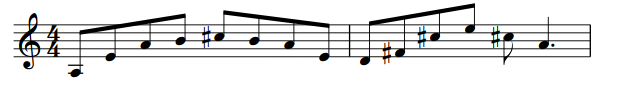
\includegraphics[width=.85\linewidth]{../code/musikla/musikla/examples/paper/concatenation2.png}}%
  }%
  \caption{Generated music sheet for concatenation\protect\footnotemark, audio version available \href{https://drive.google.com/open?id=1TP4lcul81s8iMCUFmD3HKnSpeftCzKT0}{\underline{here}}\protect\footnotemark.}
  \label{fig:concatenation}
\end{figure}

\footnotetext[\numexpr\thefootnote-1]{Rendered with \$ABC\_UI. Some hand made changes made for clarity.}
\footnotetext{\url{https://drive.google.com/open?id=1TP4lcul81s8iMCUFmD3HKnSpeftCzKT0}}


\paragraph*{Repetition}
The repetition operand is in a way very similar to the concatenation operator. It makes sense, since repeating any kind of music pattern $N$ times could be thought as a particular case of as concatenation where there are $N$ operands, all representing the same musical pattern.

\begin{lstlisting}[caption={Intro to Westworld's Theme by Ramin Djawadi},label=list:5,captionpos=t,abovecaptionskip=-\medskipamount]
I1 S6/8 T140 L/8 V90;
A*11 G F*12
\end{lstlisting}

\begin{figure}[ht]
  \centering
  {%
  \setlength{\fboxsep}{0pt}%
  \setlength{\fboxrule}{0pt}%
  \fbox{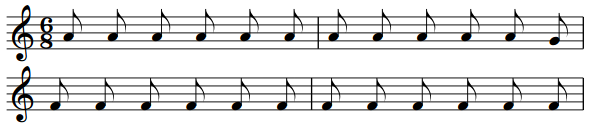
\includegraphics[width=.85\linewidth]{../code/musikla/musikla/examples/paper/repetition2.png}}%
  }%
  \caption{Generated music sheet for repetition, audio version available \href{https://drive.google.com/open?id=1IIm8PQkLsNFMK9MNSVubJSG6SP6KwhPL}{\underline{here}}\protect\footnotemark.}
  \label{fig:repetition}
\end{figure}

\footnotetext{\url{https://drive.google.com/open?id=1IIm8PQkLsNFMK9MNSVubJSG6SP6KwhPL}}

\paragraph*{Parallel}
The parallel operator enables playing multiple sequences of musical events simultaneously. However our events are emitted as a single sequence of ordered events, thus requiring merging the multiple sequences into a single one, while maintaining the properties of laziness and order. The operator assumes that each of its operands already maintains those properties on their own, and so is only in charge of making sure the merged sequence does so as well. With this in mind, it relies on a custom \textit{merge sorted} algorithm for iterables (not related to the most common merge sort algorithm by John von Neumann).

\begin{lstlisting}[caption={Snippet of the song \textit{Soft to Be Strong} by Marina},label=list:6,captionpos=t,abovecaptionskip=-\medskipamount]
T120 V70 L1;
r/4 ^g/4 ^g/4 ^g/4   ^f/2 e/8 ^d3/8   ^c2 | [^Cm] [BM]  [AM] [BM] 
\end{lstlisting}

\begin{figure}[ht]
  \centering
  {%
  \setlength{\fboxsep}{0pt}%
  \setlength{\fboxrule}{0pt}%
  \fbox{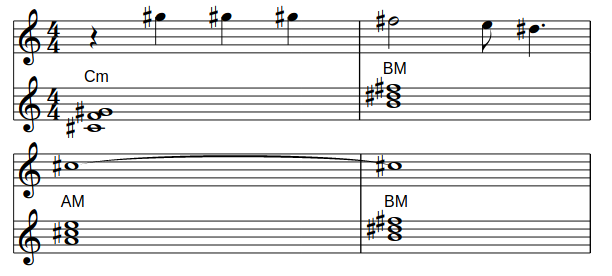
\includegraphics[width=.85\linewidth]{../code/musikla/musikla/examples/paper/parallel2.png}}%
  }%
  \caption{Generated music sheet for parallel, audio version available \href{https://drive.google.com/open?id=1ENTm3hZonYHyQIOgRZ8TQ1Qz-AfRLt2I}{\underline{here}}\protect\footnotemark.}
  \label{fig:parallel}
\end{figure}
\footnotetext{\url{https://drive.google.com/open?id=1ENTm3hZonYHyQIOgRZ8TQ1Qz-AfRLt2I}}

The merge sorted function receives $N$ operands and creates a buffer with the size $N$. For each operand it \textit{forks} the context, so that they can execute concurrently and each will mutate their own context only. It then requests one single event for each operand.

After the buffer is prefilled (meaning it has at least one event for all non-empty operands), the algorithm finds the earliest event stored in the it. Let's assume it is stored in the $K$ index of the buffer, with $K < N$. The method emits the value stored in \texttt{buffer[K]} and then fills requests the next event from the $K$ operand (storing \texttt{null} if the operand has no more events to emit). It then repeats this step until all operands have been drained.

\subsection{Integration in a Programming Environment}
Apart from generating musical events from syntatic constructs, our goal is to have those events integrate into the rest of our own DSL in the same way integers, floats, strings and booleans do: as data that can be stored, passed around and manipulated. This, of course, must still retain all the properties we've laid out for our sequences of events: being lazy and always being ordered.

\paragraph*{Variables and Functions}
All expressions that are assigned to a variable run in a forked context, with it's cursor set to zero initially. Musical expressions inside variables are still lazy (meaning they only calculate each musical event when the variable is first used, not declared) but the events are cached to prevent the calculations from being performed every time the variable is used. This cache is then garbage collected when the variable is no longer in use.

Sometimes this lazyness can indeed be more trouble than it's worth, and that's why from the very beginning the language allows the user to explicitly consume a musical sequence (with the knowledge that it cannot be an infinite one, or the application will hang). Once consumed, all it's  events will be cached in memory, stored in a list, and the user doesn't need to worry about laziness there anymore.

When events are stored in a variable, their timestamps are relative to the start timestamp of that variable (which is always zero). But when the variable is then used inside some expression, the events' timestamps must be updated to be relative to where the variable was inserted into. Since one variable can be inserted into more than one place, we cannot edit the timestamp of the event \textit{in place}, otherwise the places where we had already used that variable would have their events' timestamps changed too. This highlights the need for musical events to be immutable, and for the need to copy them when we need to make a change to one of their properties.

This works well enough because those events are very lightweight objects, and the benefits of not having their values mysteriously changed midway during execution outweight the small cost of a possible unnecessary allocation of an event that would only be used in one place instead of many.

Function calls, on the other hand, pass the current context to the inside of the function, so  that any events played there now their correct times.

When integrating functions into our language, we decided to keep the semantics simple. Returning musical events inside a function is similar to its return value being an iterator that gives out the emitted events on demand (similar to how many programming languages implement generator functions and emit values with the \textit{yield} keyword). This means that a function cannot both return musical events, while also returning other values manually through a \texttt{return} statement.

There is no syntactic marker to distinguish regular functions from \textit{"musical-emitting"} ones (meaning, there is no explicit \textit{yield} keyword). Instead, the language runtime starts executing each function as a regular one, and automatically switches its execution mode into a generator-like implementation once a statement that returns musical events is executed (and it's value is not captures into a variable). Any return statements that are evaluated after this point must have no value (thus preserving the ability to early-stop a function). If they do try to return a custom value, a runtime exception is triggered.

Here in the listing \ref{lst:fugue} we can see a small snippet of the beginning of \textit{Fugue 2 in C minor in Book I of the J.S. Bach’s Well-Tempered Clavier} written in our language, and how using functions and variables can help us visualize the structure behind music.

We also make use of the \texttt{stretch} function included in our standard library, which receives two arguments of type \textbf{Music}, and returns the first one but with it's duration proportionally stretched (or shrunk) to have the same total duration as the second musical expression.

\begin{lstlisting}[label={lst:fugue},caption={Example of repeating the same note},captionpos=t,abovecaptionskip=-\medskipamount]
fun fugue ( $subj, $resp ) => 
    ( $subj $resp | stretch( r, $subj ) ( $subj + 7 ) );

S8/4 T140 L/4 V120;

$subj = r c/2 B/2 c G _A c/2 B/2 c d
        G c/2 B/2 c d F/2 G/2 _A2 G/2 F/2;

$resp = E/2 c/2 B/2 A/2   G/2 F/2 _E/2 D/2   C _e d c
        _B A _B c   ^F G _A F;

play( fugue( $subj, $resp ) );
\end{lstlisting}


\begin{figure}[ht]
  \centering
  {%
  \setlength{\fboxsep}{0pt}%
  \setlength{\fboxrule}{0pt}%
  \fbox{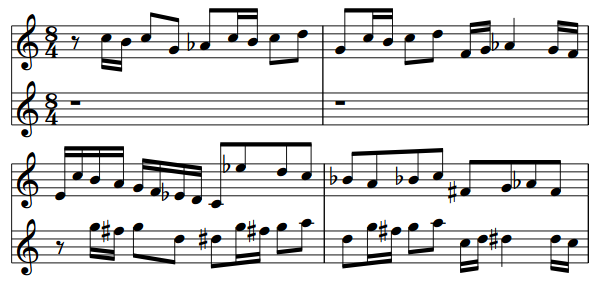
\includegraphics[width=.85\linewidth]{../code/musikla/musikla/examples/paper/fugue.png}}%
  }%
  \caption{Generated music sheet for fugue example, audio version available \href{https://drive.google.com/open?id=1dIfvnhhKn73Vpp0W6ss6RLsv6PQ_HFTF}{\underline{here}}\protect\footnotemark.}
  \label{fig:fugue}
\end{figure}
\footnotetext{\url{https://drive.google.com/open?id=1dIfvnhhKn73Vpp0W6ss6RLsv6PQ_HFTF}}

The music sheet generated by the code in the listing~\ref{lst:fugue} can be seen in figure~\ref{fig:fugue}. The two staves of the first system correspond to the expressions \texttt{\$subj} and \texttt{stretch( r, \$subj )}, respectively (we can identify it easily in the second staff, where there are only rests). The two staves of the second system on the other hand, correspond to the expressions \texttt{\$resp} and \texttt{( \$subj + 7 )} (the later of the two being a transposition of \texttt{\$subj} but with a higher pitch of 7 semitones).

\paragraph*{Grids}
To define a grid there is only one parameter required: the length of it's cells. When aligning musical events, anything that falls inside each cell will be pushed to the closest edge of the cell.

Grids are highly customizable too, however. They have multiple parameters, such as \texttt{forgiveness} and \texttt{range}, that determine when an event is affected by the grid (depending on how close it's start time is to the edge of the cell). Each parameter can even be customized separately for the left and right sides of the cell's edge.

Let's take a look at an example of a grid. In this example the grid has a cell size of \textbf{1}. We define the same values for both left and right sides just for the sake of this demonstration, but each side could have different values.

\begin{lstlisting}[caption={Declaring a grid},label=list:8,captionpos=t,abovecaptionskip=-\medskipamount]
$grid = Grid( 1,
    forgiveness_left = 125, # 1/8
    range_left = 375, # 3/8
    forgiveness_right = 125, #1/8
    range_right = 375 # 3/8
);
\end{lstlisting}

\begin{figure}[ht]
  \centering
  {%
  \setlength{\fboxsep}{0pt}%
  \setlength{\fboxrule}{0pt}%
  \fbox{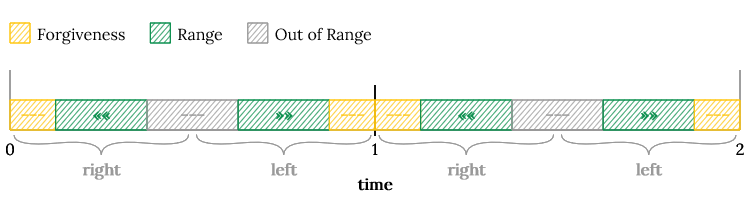
\includegraphics[width=.95\linewidth]{./img/grids.png}}%
  }%
  \caption{Representation of two cells from this grid.}
  \label{fig:grid}
\end{figure}

We can see in this timeline two cells (each with a size of 1). Any events that fall in the yellow and grey areas are ignored (meaning their timestamps are not changed) while events in the green areas are pushed to whatever edge is closest. But even this behavior can be customized, forcing events to always go to the previous edge cell, or always to the next.

It is then trivial to see how we could compose multiple grids in sequence, each with different ranges (green areas) that capture different events and align them accordingly.

\paragraph*{Keyboards}
Finally we can combine all the systems we've described above, from musical expressions, grids, variables and functions, and devise a compact way of describing virtual keyboards.

To make the process of designing keyboards less verbose, we've added syntactic sugar to this process, that is translated in the background to regular function calls registering each key binding.

While a picture maybe worth a thousand words, a good example is worth maybe even more. So here we can take a brief look at the workflow for defining two keyboards (that are active at the same time). The first keyboard has all the musical keys (the chords and single notes we want), all aligned by a custom grid.

The second keyboard binds to the up and down arrow keys and allow us to change the virtual instrument through which we play the sounds of the notes in the keyboard (those instruments can be identified by an integer and usually follow the General MIDI standard\cite{GeneralMIDI}).

\begin{lstlisting}[caption={Creating a keyboard that can play multiple instruments},label=list:9,captionpos=t,abovecaptionskip=-\medskipamount]
$inst = 0;

fun spin_instrument ( ref $instrument, $change ) {
    $instrument = $instrument + $change;
    
    setinstrument( $instrument );
};

@keyboard {
    a: [^Cm];   s: [BM];    d: [AM];    f: [EM];    g: [^Fm];
    1: ^c;      2: ^d;      3: e;       4: ^f;      5: ^g;
    6: b;       7: ^c';     8: ^d';     9: e';
}::with_grid( Grid( 1 / 16 ) );

@keyboard {
    up: spin_instrument( $inst, 1 );
    down: spin_instrument( $inst, -1 );
};
\end{lstlisting}

Keyboards are objects (that we could save in a variable for example) and that can perform many operations, like unions and intersections, or maps and filters. They can be enabled and disabled at runtime, and their keys can be simulated to be pressed and released.

More than that, we don't need to restrict ourselves to computer keyboards. We can for instance, define bindings between MIDI events and musical expressions, so that when we connect a piano keyboard to our computer, we can use each piano key to play more than a single note.

Since like we've seen keyboard keys are not limited to computer keyboards, we can imagine the possibilities of events we could listen to: knobs, mouse buttons, the mouse scroll wheel. We could even create an event that could, for example, listen on a socket and trigger when a message is received, allowing in that way our musical applications to be controlled remotely.

The result is that our keyboards are extremely extensible and allow for a great deal of creativity. And thanks to our tight integration with the Python language, those extensions can be easily integrated and don't require hacking the source code or recompiling the application.

\section{Results Discussion and Conclusion}
\label{sec:conclusions}

The scope of this project could have been massive, mainly because implementing a way to fully describe hundreds of years of comulative musical notation would be a gigantic task. We chose instead to build a solid foundation, always with a strong focus on extensibility for the future.

This hability to extend the functionality of our project, thanks to our easy integration with regular Python code, means that new types of musical events, new inputs or outputs, new functions or libraries can be added with minimal effort by everyone using our application. There is no need to recompile the project or change the source, just include the \textit{Python} code at runtime.

When it comes to keyboards, there are many more possibilities to explore too. While we've included  examples of working with key presses, both from computer keyboards as well as pianos (through a MIDI connection), more rich events can also be used that were not demonstrated here. Since each event can also carry parameters with it, we can do more than boolean press/release types of events: we can model knobs or scroll wheels or other kinds of spatial events into our keyboards.

A work in progress implementation of the project can be found on GitHub\footnote{\url{https://github.com/pedromsilvapt/miei-dissertation}}, with an online work-in-progress documentation available as well\footnote{\url{https://pedromsilvapt.github.io/miei-dissertation/}}. It is possible that a more stable version can be published to the Python Package Index (PyPi) somewhere in the near future.

The current version is already very usable in practice, which can be seen both in the examples provided in this paper (alongside with the generated audio and music sheets, both created by our application already) as well as many different experiments that have already been developed during this dissertation. We do think in our (obviously biased) humble opinion that the project has a lot of potential, particularly to serve as a swiss army knife, extensible and customizable solution for music creation and experimentation.

\bibliography{references}
\end{document}
